\chapter{Mô Tả Thiết Kế Phần Mềm}

\section{Thiết Kế Hệ Thống}

\subsection{Kiến Trúc Hệ Thống}

\subsection{Sơ Đồ Package}

\section{Thiết Kế Cơ Sở Dữ Liệu}

\subsection{Sơ Đồ Thực Thể Quan Hệ}

\begin{figure}[H]
  \centering
  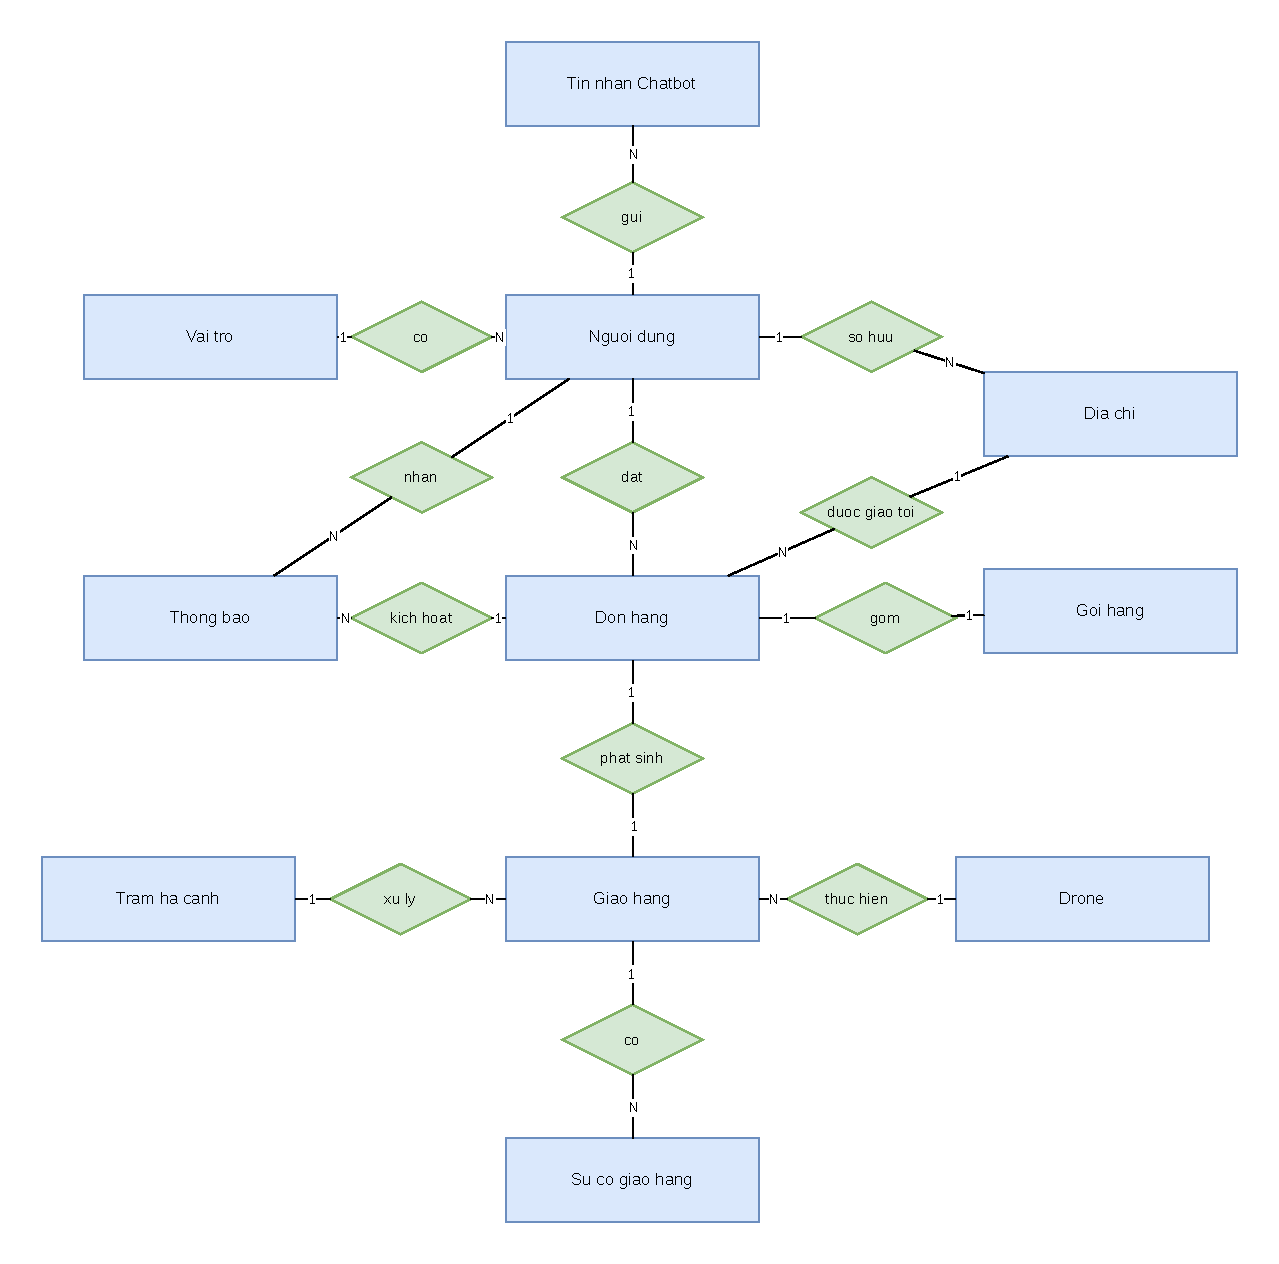
\includegraphics[width=\textwidth]{so-do/ERD.pdf}
  \caption{Sơ đồ thực thể quan hệ của hệ thống SmartDroneDelivery}
  \label{fig:erd}
\end{figure}

\subsection{Mô Tả Chi Tiết Các Bảng}

\begin{table}[H]
  \centering
  \begin{tabularx}{\textwidth}{|l|l|l|>{\raggedright\arraybackslash}X|}
    \hline
    \textbf{Tên cột} & \textbf{Kiểu dữ liệu} & \textbf{Ràng buộc} & \textbf{Mô tả} \\
    \hline
    ma\_vai\_tro         & UUID            & PK, NOT NULL    & Mã vai trò (tự động tạo UUID) \\ \hline
    ten\_vai\_tro        & VARCHAR(50)     & NOT NULL, UNIQUE & Tên vai trò (Admin, Dispatcher, v.v.) \\ \hline
    created\_at          & TIMESTAMPTZ     & NOT NULL        & Thời gian tạo bản ghi \\ \hline
    updated\_at          & TIMESTAMPTZ     & NOT NULL        & Thời gian cập nhật bản ghi \\
    \hline
  \end{tabularx}
  \caption{Cấu trúc bảng \texttt{vai\_tro} (Vai trò người dùng)}
  \label{tab:db-vai-tro}
\end{table}

\begin{table}[H]
  \centering
  \begin{tabularx}{\textwidth}{|l|l|l|>{\raggedright\arraybackslash}X|}
    \hline
    \textbf{Tên cột} & \textbf{Kiểu dữ liệu} & \textbf{Ràng buộc} & \textbf{Mô tả} \\
    \hline
    ma\_nguoi\_dung      & UUID            & PK, NOT NULL    & Mã người dùng (tự động tạo UUID) \\ \hline
    ma\_vai\_tro         & UUID            & FK, NOT NULL    & Khóa ngoại tham chiếu đến bảng vai\_tro \\ \hline
    ho\_ten              & VARCHAR(150)    & NOT NULL        & Họ và tên người dùng \\ \hline
    email                & VARCHAR(255)    & NOT NULL, UNIQUE & Địa chỉ email người dùng \\ \hline
    so\_dien\_thoai      & VARCHAR(20)     & NULL            & Số điện thoại liên hệ \\ \hline
    mat\_khau\_hash      & TEXT            & NOT NULL        & Mật khẩu đã mã hóa hash \\ \hline
    ngay\_tao            & TIMESTAMPTZ     & NOT NULL        & Ngày giờ tạo tài khoản \\ \hline
    updated\_at          & TIMESTAMPTZ     & NOT NULL        & Thời gian cập nhật gần nhất \\
    \hline
  \end{tabularx}
  \caption{Cấu trúc bảng \texttt{nguoi\_dung} (Tài khoản người dùng)}
  \label{tab:db-nguoi-dung}
\end{table}

\begin{table}[H]
  \centering
  \begin{tabularx}{\textwidth}{|l|l|l|>{\raggedright\arraybackslash}X|}
    \hline
    \textbf{Tên cột} & \textbf{Kiểu dữ liệu} & \textbf{Ràng buộc} & \textbf{Mô tả} \\
    \hline
    ma\_kh               & UUID            & PK, NOT NULL    & Mã khách hàng (tự động tạo UUID) \\ \hline
    ten                  & VARCHAR(50)     & NOT NULL        & Tên khách hàng \\ \hline
    ten\_dem             & VARCHAR(50)     & NULL            & Tên đệm \\ \hline
    ho                   & VARCHAR(50)     & NOT NULL        & Họ của khách hàng \\ \hline
    gioi\_tinh           & VARCHAR(10)     & CHECK           & Giới tính (Nam, Nữ, Khác) \\ \hline
    so\_dien\_thoai      & VARCHAR(20)     & NULL            & Số điện thoại liên hệ \\ \hline
    email                & VARCHAR(255)    & UNIQUE          & Địa chỉ email khách hàng \\ \hline
    ngay\_sinh           & DATE            & NULL            & Ngày tháng năm sinh \\ \hline
    created\_at          & TIMESTAMPTZ     & NOT NULL        & Thời gian tạo bản ghi \\ \hline
    updated\_at          & TIMESTAMPTZ     & NOT NULL        & Thời gian cập nhật bản ghi \\
    \hline
  \end{tabularx}
  \caption{Cấu trúc bảng \texttt{khach\_hang} (Thông tin khách hàng)}
  \label{tab:db-khach-hang}
\end{table}

\begin{table}[H]
  \centering
  \begin{tabularx}{\textwidth}{|l|l|l|>{\raggedright\arraybackslash}X|}
    \hline
    \textbf{Tên cột} & \textbf{Kiểu dữ liệu} & \textbf{Ràng buộc} & \textbf{Mô tả} \\
    \hline
    ma\_dia\_chi         & UUID            & PK, NOT NULL    & Mã địa chỉ (tự động tạo UUID) \\ \hline
    ma\_kh               & UUID            & FK, NOT NULL    & Khóa ngoại tham chiếu đến bảng khach\_hang \\ \hline
    dia\_chi\_cu\_the    & TEXT            & NOT NULL        & Địa chỉ chi tiết (số nhà, tên đường) \\ \hline
    thanh\_pho           & VARCHAR(100)    & NOT NULL        & Tên tỉnh hoặc thành phố \\ \hline
    lat                  & DOUBLE          & NOT NULL        & Vĩ độ GPS trên bản đồ \\ \hline
    lng                  & DOUBLE          & NOT NULL        & Kinh độ GPS trên bản đồ \\ \hline
    created\_at          & TIMESTAMPTZ     & NOT NULL        & Thời gian tạo bản ghi \\ \hline
    updated\_at          & TIMESTAMPTZ     & NOT NULL        & Thời gian cập nhật bản ghi \\
    \hline
  \end{tabularx}
  \caption{Cấu trúc bảng \texttt{dia\_chi} (Địa chỉ giao hàng)}
  \label{tab:db-dia-chi}
\end{table}

\begin{table}[H]
  \centering
  \begin{tabularx}{\textwidth}{|l|l|l|>{\raggedright\arraybackslash}X|}
    \hline
    \textbf{Tên cột} & \textbf{Kiểu dữ liệu} & \textbf{Ràng buộc} & \textbf{Mô tả} \\
    \hline
    ma\_tin\_nhan        & UUID            & PK, NOT NULL    & Mã tin nhắn (tự động tạo UUID) \\ \hline
    ma\_kh               & UUID            & FK, NOT NULL    & Khóa ngoại tham chiếu đến bảng khach\_hang \\ \hline
    noi\_dung            & TEXT            & NOT NULL        & Nội dung tin nhắn khách hàng gửi \\ \hline
    phan\_hoi            & TEXT            & NULL            & Nội dung phản hồi từ Chatbot AI \\ \hline
    thoi\_gian           & TIMESTAMPTZ     & NOT NULL        & Thời gian gửi tin nhắn \\
    \hline
  \end{tabularx}
  \caption{Cấu trúc bảng \texttt{tin\_nhan\_chatbot} (Lịch sử chat AI)}
  \label{tab:db-tin-nhan-chatbot}
\end{table}

\begin{table}[H]
  \centering
  \begin{tabularx}{\textwidth}{|l|l|l|>{\raggedright\arraybackslash}X|}
    \hline
    \textbf{Tên cột} & \textbf{Kiểu dữ liệu} & \textbf{Ràng buộc} & \textbf{Mô tả} \\
    \hline
    ma\_don\_hang        & UUID            & PK, NOT NULL    & Mã đơn hàng (tự động tạo UUID) \\ \hline
    ma\_kh               & UUID            & FK, NOT NULL    & Khóa ngoại tham chiếu đến bảng khach\_hang \\ \hline
    ma\_dia\_chi         & UUID            & FK, NOT NULL    & Khóa ngoại tham chiếu đến bảng dia\_chi \\ \hline
    trang\_thai\_don\_hang & VARCHAR(30)     & NOT NULL, CHECK & Trạng thái đơn (Chờ duyệt, Đã duyệt, Đang giao, v.v.) \\ \hline
    cach\_thuc\_thanh\_toan & VARCHAR(50)     & NULL            & Phương thức thanh toán \\ \hline
    tong\_tien           & DECIMAL(15,2)   & DEFAULT 0       & Tổng giá trị đơn hàng \\ \hline
    ngay\_dat\_hang      & TIMESTAMPTZ     & NOT NULL        & Ngày giờ đặt đơn hàng \\ \hline
    ngay\_cap\_nhat      & TIMESTAMPTZ     & NOT NULL        & Thời gian cập nhật gần nhất \\
    \hline
  \end{tabularx}
  \caption{Cấu trúc bảng \texttt{don\_hang} (Đơn hàng giao)}
  \label{tab:db-don-hang}
\end{table}

\begin{table}[H]
  \centering
  \begin{tabularx}{\textwidth}{|l|l|l|>{\raggedright\arraybackslash}X|}
    \hline
    \textbf{Tên cột} & \textbf{Kiểu dữ liệu} & \textbf{Ràng buộc} & \textbf{Mô tả} \\
    \hline
    ma\_tram             & UUID            & PK, NOT NULL    & Mã trạm hạ cánh (tự động tạo UUID) \\ \hline
    ten\_tram            & VARCHAR(150)    & NOT NULL        & Tên trạm hạ cánh \\ \hline
    dia\_chi\_tram       & TEXT            & NOT NULL        & Địa chỉ chi tiết của trạm \\ \hline
    lat                  & DOUBLE          & NOT NULL        & Vĩ độ GPS của trạm \\ \hline
    lng                  & DOUBLE          & NOT NULL        & Kinh độ GPS của trạm \\ \hline
    cong\_suat\_toi\_da  & INT             & NOT NULL        & Sức chứa hoặc công suất tối đa của trạm \\ \hline
    trang\_thai\_hoat\_dong & VARCHAR(20)     & NOT NULL, CHECK & Trạng thái trạm (Đang hoạt động, Bảo trì, Ngừng) \\ \hline
    created\_at          & TIMESTAMPTZ     & NOT NULL        & Thời gian tạo bản ghi \\ \hline
    updated\_at          & TIMESTAMPTZ     & NOT NULL        & Thời gian cập nhật bản ghi \\
    \hline
  \end{tabularx}
  \caption{Cấu trúc bảng \texttt{tram\_ha\_canh} (Trạm hạ cánh drone)}
  \label{tab:db-tram-ha-canh}
\end{table}

\begin{table}[H]
  \centering
  \begin{tabularx}{\textwidth}{|l|l|l|>{\raggedright\arraybackslash}X|}
    \hline
    \textbf{Tên cột} & \textbf{Kiểu dữ liệu} & \textbf{Ràng buộc} & \textbf{Mô tả} \\
    \hline
    ma\_goi\_hang        & UUID            & PK, NOT NULL    & Mã gói hàng (tự động tạo UUID) \\ \hline
    ma\_don\_hang        & UUID            & FK, NOT NULL    & Khóa ngoại tham chiếu đến bảng don\_hang \\ \hline
    ma\_tram             & UUID            & FK, NULL        & Khóa ngoại tham chiếu đến bảng tram\_ha\_canh \\ \hline
    loai\_hang\_hoa      & VARCHAR(100)    & NOT NULL        & Loại hàng hóa trong gói \\ \hline
    can\_nang            & DECIMAL(8,2)    & NOT NULL, CHECK & Cân nặng gói hàng (tối đa 5kg) \\ \hline
    kich\_co             & VARCHAR(50)     & NULL            & Kích thước gói hàng \\ \hline
    gia\_tri\_uoc\_tinh  & DECIMAL(15,2)   & DEFAULT 0       & Giá trị ước tính của gói hàng \\ \hline
    created\_at          & TIMESTAMPTZ     & NOT NULL        & Thời gian tạo bản ghi \\ \hline
    updated\_at          & TIMESTAMPTZ     & NOT NULL        & Thời gian cập nhật bản ghi \\
    \hline
  \end{tabularx}
  \caption{Cấu trúc bảng \texttt{goi\_hang} (Gói hàng vận chuyển)}
  \label{tab:db-goi-hang}
\end{table}

\begin{table}[H]
  \centering
  \begin{tabularx}{\textwidth}{|l|l|l|>{\raggedright\arraybackslash}X|}
    \hline
    \textbf{Tên cột} & \textbf{Kiểu dữ liệu} & \textbf{Ràng buộc} & \textbf{Mô tả} \\
    \hline
    ma\_drone            & UUID            & PK, NOT NULL    & Mã thiết bị drone (tự động tạo UUID) \\ \hline
    trang\_thai\_drone   & VARCHAR(30)     & NOT NULL, CHECK & Trạng thái drone (Sẵn sàng, Đang giao, Bảo trì, Hỏng) \\ \hline
    cong\_suat\_pin      & INT             & NOT NULL, CHECK & Dung lượng pin còn lại (0 đến 100 percent) \\ \hline
    ngay\_bao\_tri\_gan\_nhat & TIMESTAMPTZ     & NULL            & Ngày bảo trì thiết bị gần nhất \\ \hline
    created\_at          & TIMESTAMPTZ     & NOT NULL        & Thời gian tạo bản ghi \\ \hline
    updated\_at          & TIMESTAMPTZ     & NOT NULL        & Thời gian cập nhật bản ghi \\
    \hline
  \end{tabularx}
  \caption{Cấu trúc bảng \texttt{drone} (Thiết bị drone giao hàng)}
  \label{tab:db-drone}
\end{table}

\begin{table}[H]
  \centering
  \begin{tabularx}{\textwidth}{|l|l|l|>{\raggedright\arraybackslash}X|}
    \hline
    \textbf{Tên cột} & \textbf{Kiểu dữ liệu} & \textbf{Ràng buộc} & \textbf{Mô tả} \\
    \hline
    ma\_giao\_hang       & UUID            & PK, NOT NULL    & Mã chuyến giao hàng (tự động tạo UUID) \\ \hline
    ma\_don\_hang        & UUID            & FK, NOT NULL    & Khóa ngoại tham chiếu đến bảng don\_hang \\ \hline
    ma\_drone            & UUID            & FK, NULL        & Khóa ngoại tham chiếu đến bảng drone \\ \hline
    ma\_nguoi\_phu\_trach & UUID            & FK, NULL        & Khóa ngoại tham chiếu đến bảng nguoi\_dung \\ \hline
    trang\_thai\_giao\_hang & VARCHAR(30)     & NOT NULL, CHECK & Trạng thái giao (Chờ xử lý, Đang giao, Đã giao, Giao thất bại) \\ \hline
    vi\_tri\_hien\_tai\_lat & DOUBLE          & NULL            & Vĩ độ vị trí hiện tại của drone \\ \hline
    vi\_tri\_hien\_tai\_lng & DOUBLE          & NULL            & Kinh độ vị trí hiện tại của drone \\ \hline
    thoi\_gian\_giao     & TIMESTAMPTZ     & NULL            & Thời gian giao hàng thành công \\ \hline
    created\_at          & TIMESTAMPTZ     & NOT NULL        & Thời gian tạo bản ghi \\ \hline
    updated\_at          & TIMESTAMPTZ     & NOT NULL        & Thời gian cập nhật bản ghi \\
    \hline
  \end{tabularx}
  \caption{Cấu trúc bảng \texttt{giao\_hang} (Chuyến giao hàng)}
  \label{tab:db-giao-hang}
\end{table}

\begin{table}[H]
  \centering
  \begin{tabularx}{\textwidth}{|l|l|l|>{\raggedright\arraybackslash}X|}
    \hline
    \textbf{Tên cột} & \textbf{Kiểu dữ liệu} & \textbf{Ràng buộc} & \textbf{Mô tả} \\
    \hline
    ma\_van\_de          & UUID            & PK, NOT NULL    & Mã sự cố (tự động tạo UUID) \\ \hline
    ma\_tram             & UUID            & FK, NULL        & Khóa ngoại tham chiếu đến bảng tram\_ha\_canh \\ \hline
    ma\_giao\_hang       & UUID            & FK, NOT NULL    & Khóa ngoại tham chiếu đến bảng giao\_hang \\ \hline
    thoi\_gian\_xay\_ra  & TIMESTAMPTZ     & NOT NULL        & Thời gian phát sinh sự cố \\ \hline
    mo\_ta\_su\_co       & TEXT            & NOT NULL        & Mô tả chi tiết nguyên nhân và sự cố \\ \hline
    muc\_do\_nghiem\_trong & VARCHAR(20)     & NOT NULL, CHECK & Mức độ sự cố (Thấp, Trung bình, Cao, Nghiêm trọng) \\ \hline
    created\_at          & TIMESTAMPTZ     & NOT NULL        & Thời gian tạo bản ghi \\
    \hline
  \end{tabularx}
  \caption{Cấu trúc bảng \texttt{su\_co\_giao\_hang} (Ghi nhận sự cố)}
  \label{tab:db-su-co-giao-hang}
\end{table}

\begin{table}[H]
  \centering
  \begin{tabularx}{\textwidth}{|l|l|l|>{\raggedright\arraybackslash}X|}
    \hline
    \textbf{Tên cột} & \textbf{Kiểu dữ liệu} & \textbf{Ràng buộc} & \textbf{Mô tả} \\
    \hline
    ma\_thong\_bao       & UUID            & PK, NOT NULL    & Mã thông báo (tự động tạo UUID) \\ \hline
    ma\_kh               & UUID            & FK, NOT NULL    & Khóa ngoại tham chiếu đến bảng khach\_hang \\ \hline
    ma\_don\_hang        & UUID            & FK, NULL        & Khóa ngoại tham chiếu đến bảng don\_hang \\ \hline
    trang\_thai          & VARCHAR(20)     & NOT NULL, CHECK & Trạng thái thông báo (Chưa đọc, Đã đọc) \\ \hline
    thoi\_gian\_gui      & TIMESTAMPTZ     & NOT NULL        & Thời gian gửi thông báo \\ \hline
    noi\_dung            & TEXT            & NOT NULL        & Nội dung chi tiết thông báo \\
    \hline
  \end{tabularx}
  \caption{Cấu trúc bảng \texttt{thong\_bao} (Thông báo cho khách hàng)}
  \label{tab:db-thong-bao}
\end{table}

\section{Thiết Kế Chi Tiết}

\subsection{Chức Năng Đăng Nhập}
\subsubsection{Sơ Đồ Lớp}
\subsubsection{Sơ Đồ Tuần Tự}
\begin{figure}[H]
  \centering
  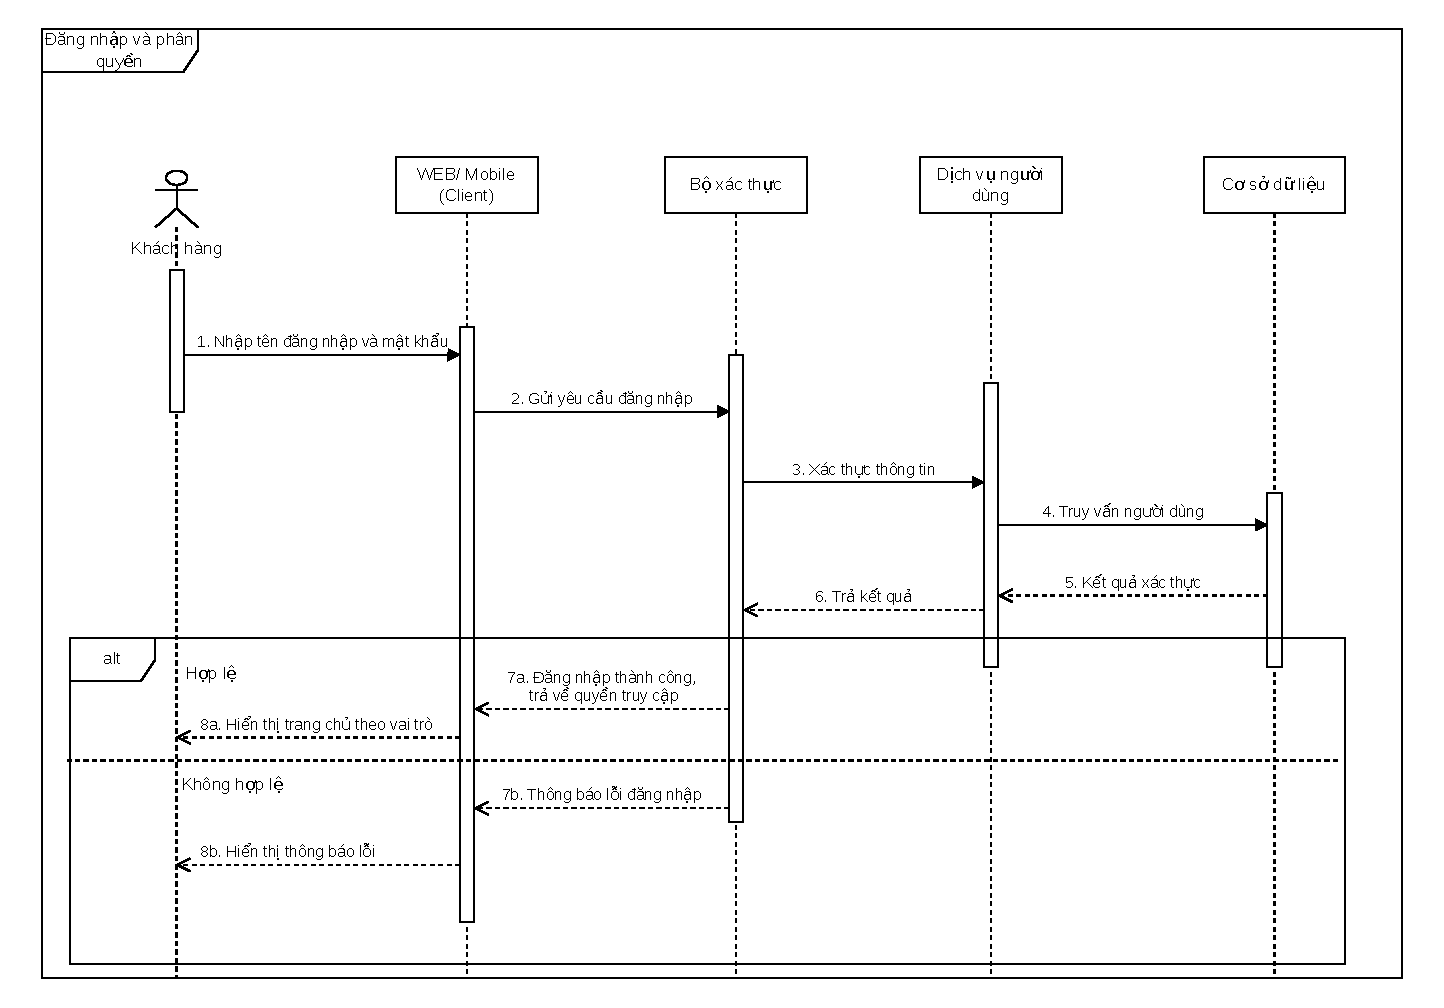
\includegraphics[width=\textwidth]{so-do/sodo-tuantu/Đăng nhập và phân quyền.drawio.pdf}
  \caption{Sơ đồ tuần tự chức năng Đăng nhập và phân quyền}
  \label{fig:seq-dangnhap}
\end{figure}

\subsection{Chức Năng Tạo Đơn Hàng Giao}
\subsubsection{Sơ Đồ Lớp}
\subsubsection{Sơ Đồ Tuần Tự}
\begin{figure}[H]
  \centering
  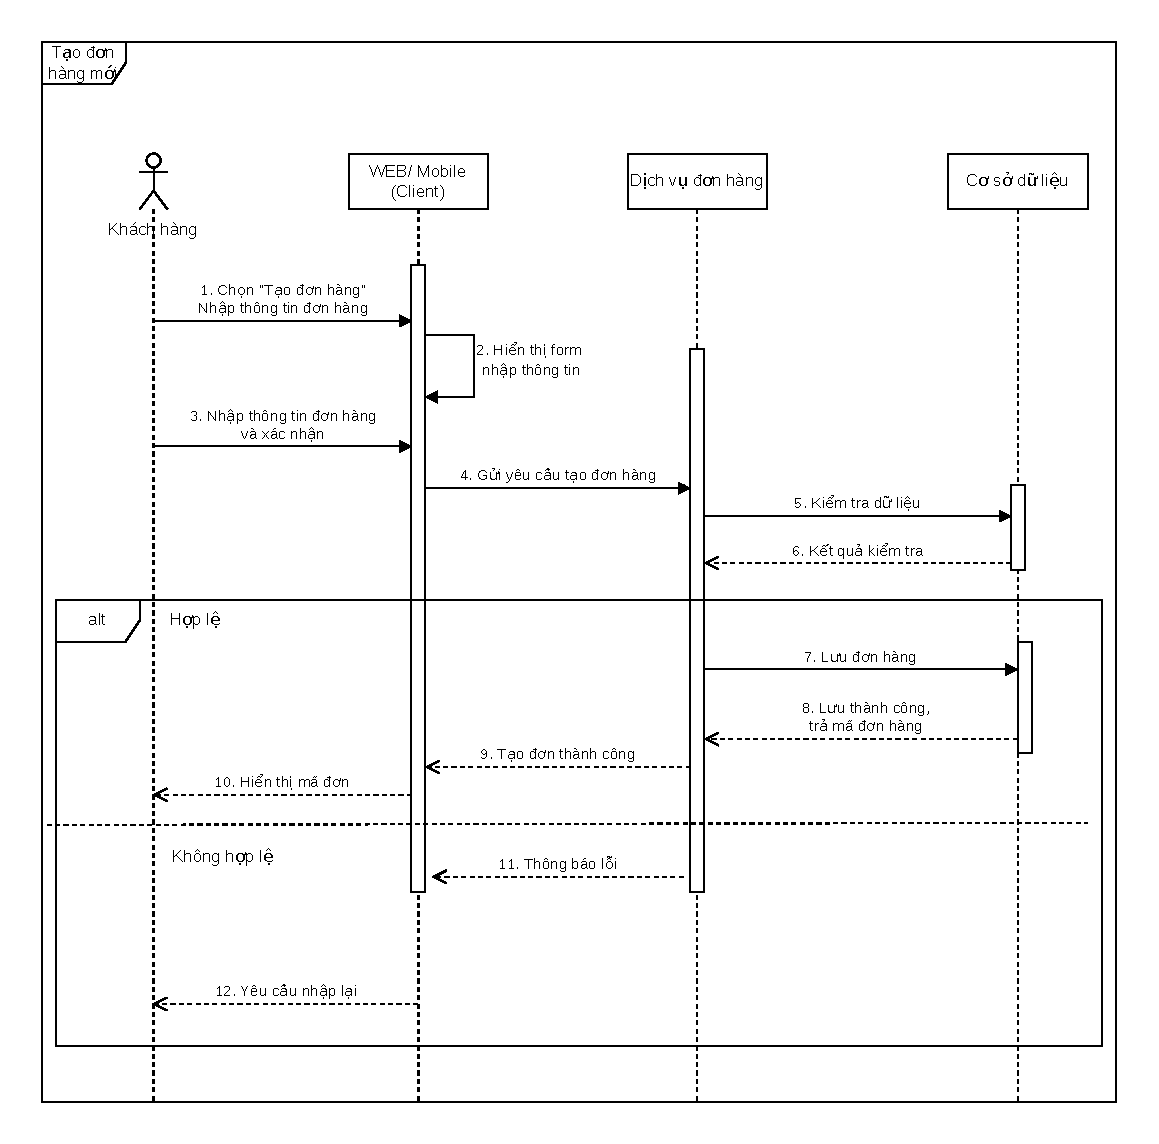
\includegraphics[width=\textwidth]{so-do/sodo-tuantu/Tạo đơn hàng mới.drawio.pdf}
  \caption{Sơ đồ tuần tự chức năng Tạo đơn hàng mới}
  \label{fig:seq-taodon}
\end{figure}

\subsection{Chức Năng Cập Nhật và Hủy Đơn Hàng}
\subsubsection{Sơ Đồ Lớp}
\subsubsection{Sơ Đồ Tuần Tự}
\begin{figure}[H]
  \centering
  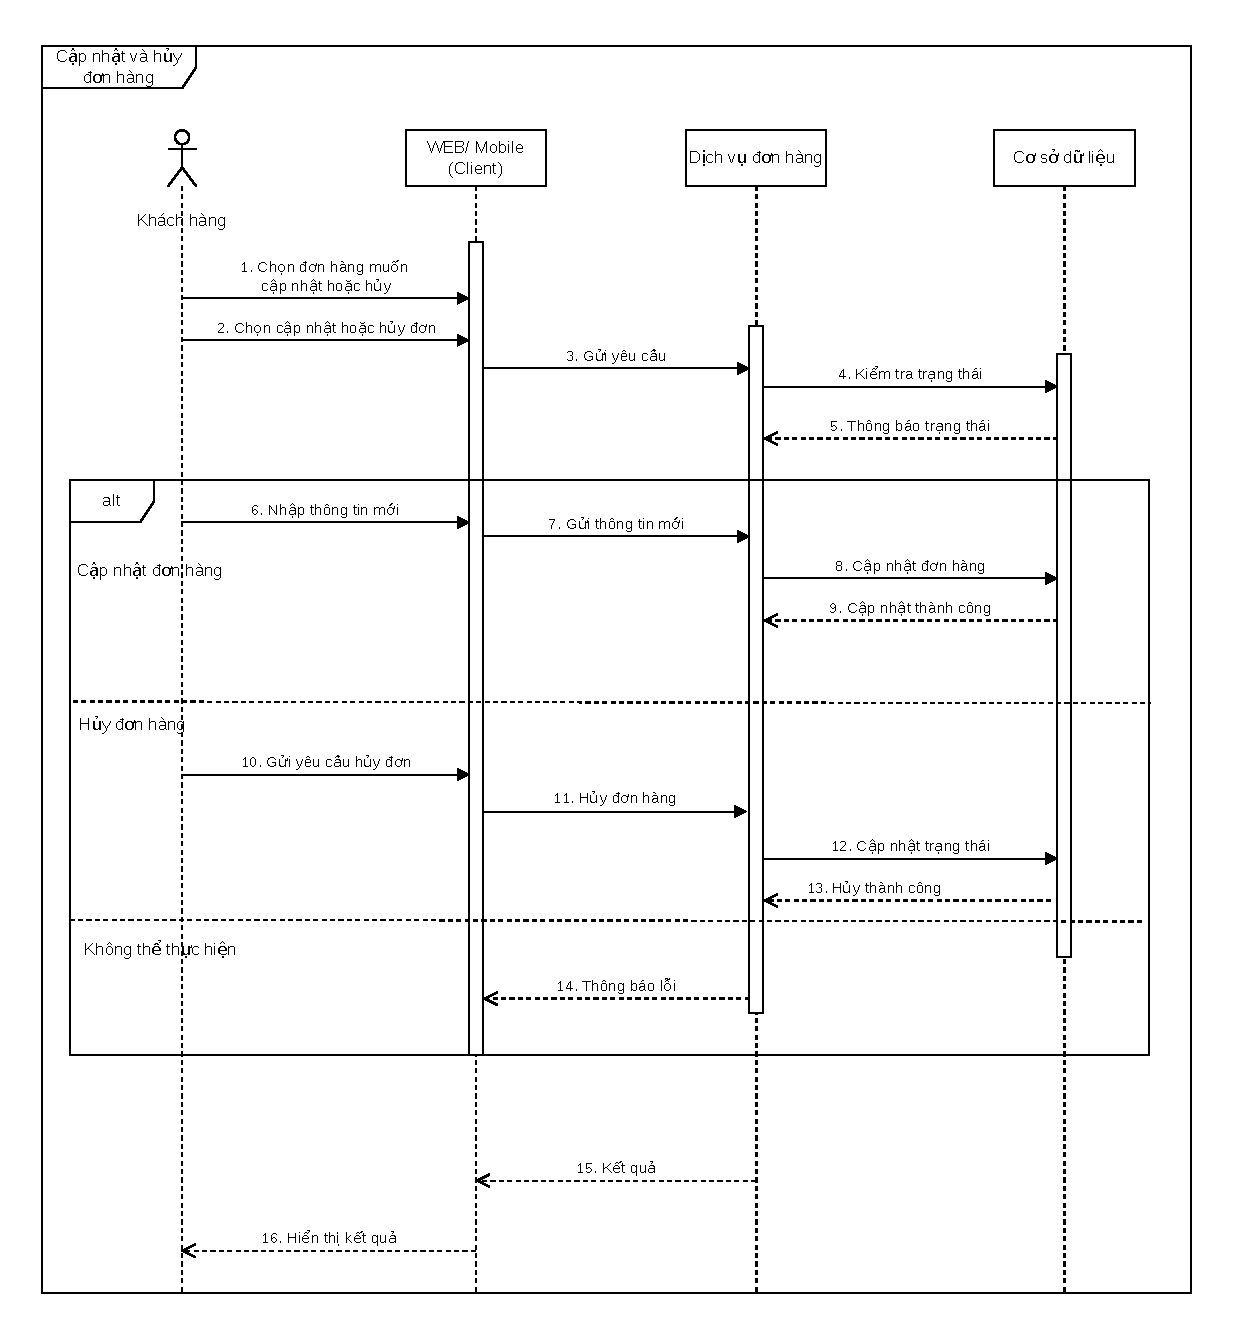
\includegraphics[width=\textwidth]{so-do/sodo-tuantu/Cập nhật và hủy đơn hàng.drawio.pdf}
  \caption{Sơ đồ tuần tự chức năng Cập nhật và hủy đơn hàng}
  \label{fig:seq-capnhat-huydon}
\end{figure}

\subsection{Chức Năng Xác Nhận và Gửi Kiện Hàng Tại Trạm}
\subsubsection{Sơ Đồ Lớp}
\subsubsection{Sơ Đồ Tuần Tự}
\begin{figure}[H]
  \centering
  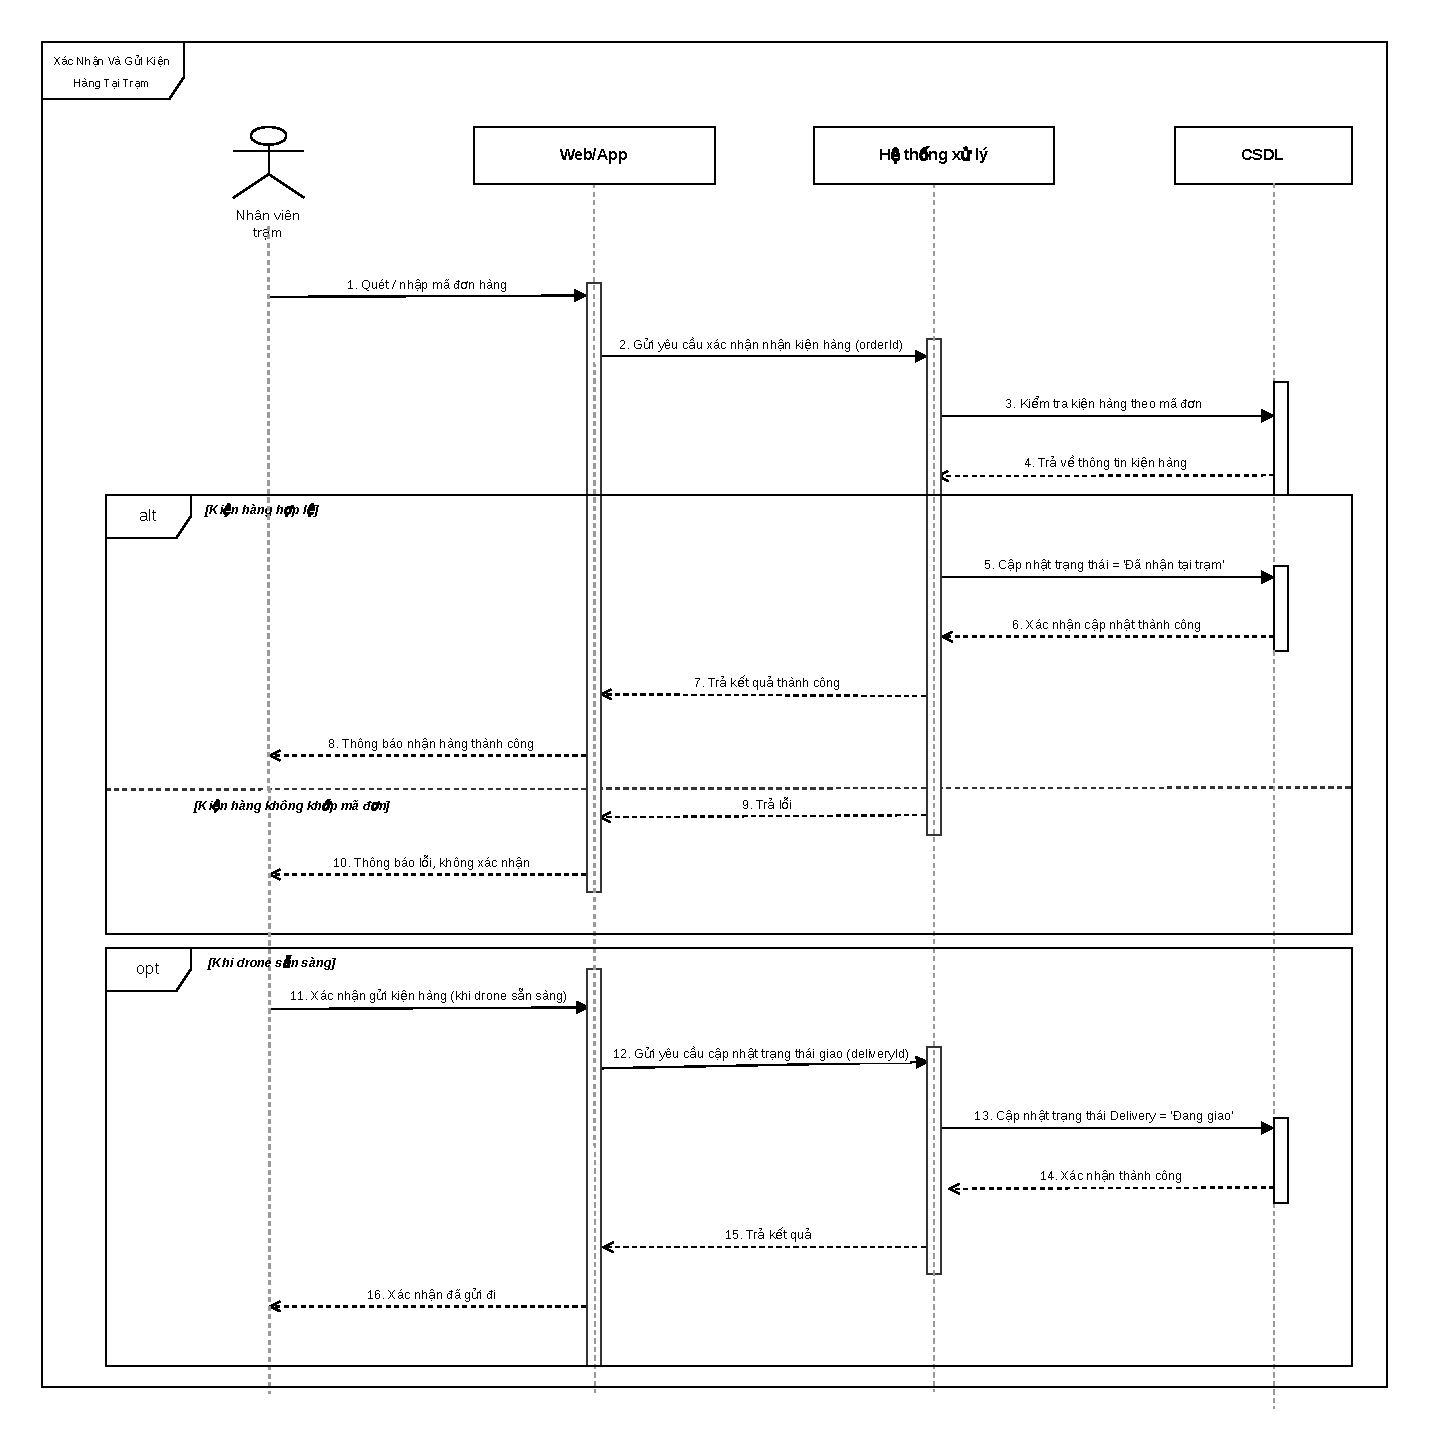
\includegraphics[width=\textwidth]{so-do/sodo-tuantu/Xác Nhận Nhận_Gửi Kiện Hàng Tại Trạm.drawio.pdf}
  \caption{Sơ đồ tuần tự chức năng Xác nhận nhận và gửi kiện hàng tại trạm}
  \label{fig:seq-xacnhan-gui-tram}
\end{figure}

\subsection{Chức Năng Theo Dõi Giao Hàng Theo Thời Gian Thực}
\subsubsection{Sơ Đồ Lớp}
\subsubsection{Sơ Đồ Tuần Tự}
\begin{figure}[H]
  \centering
  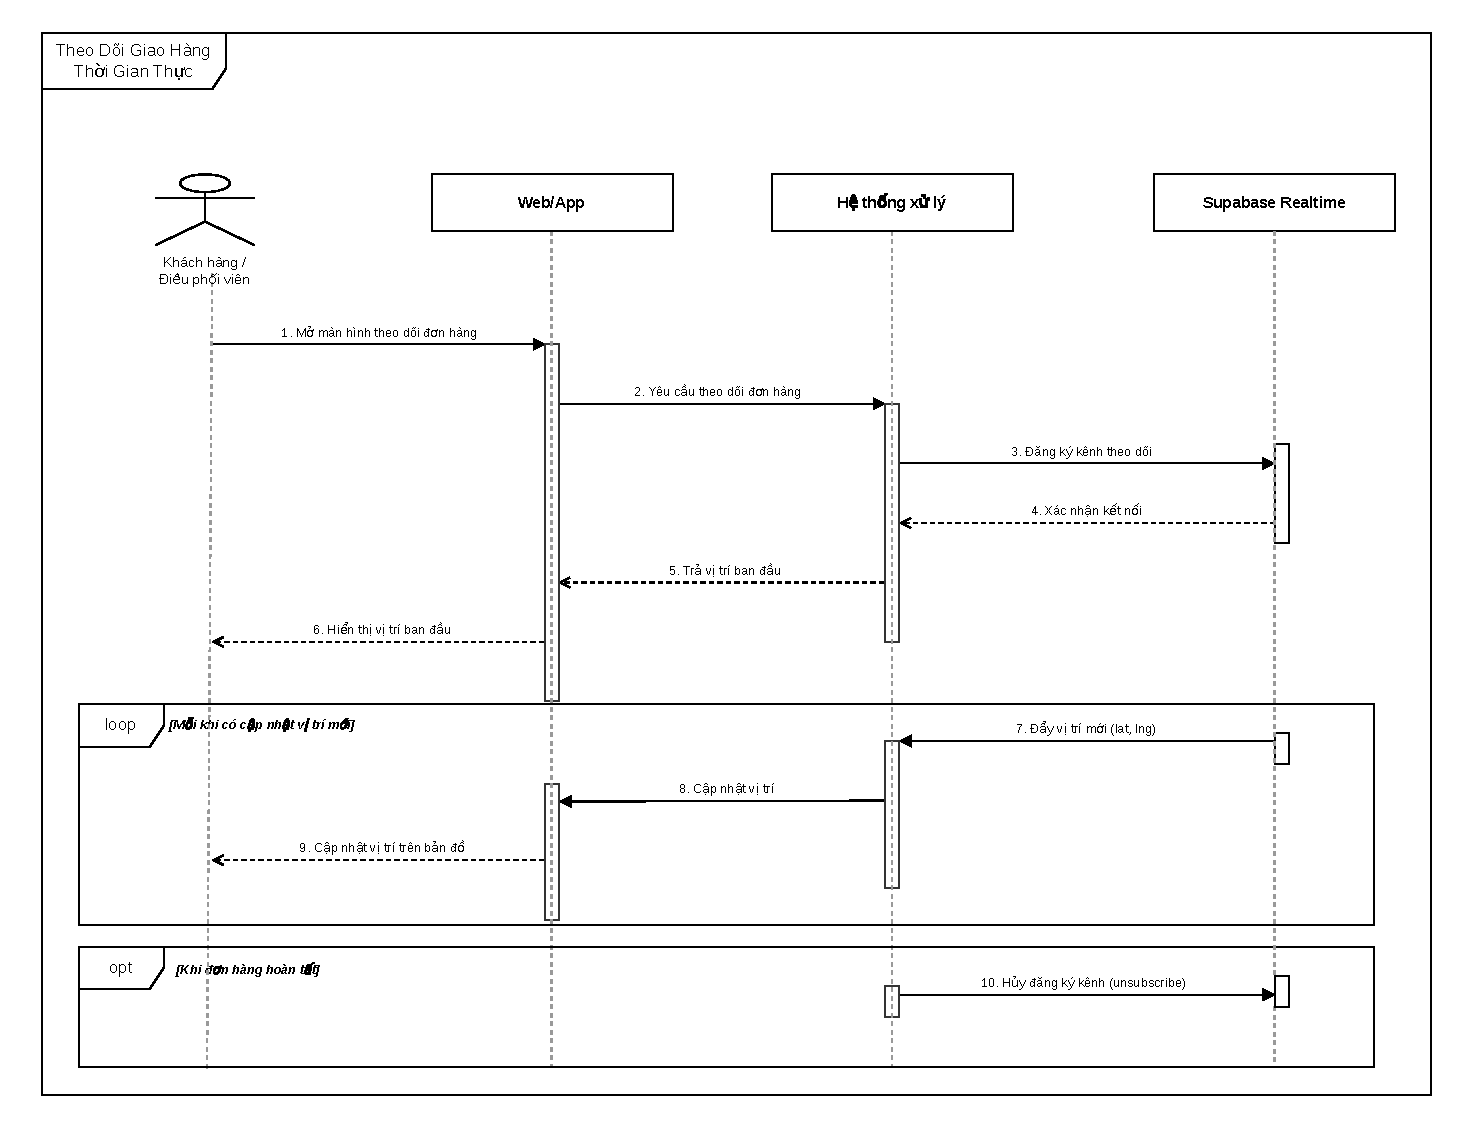
\includegraphics[width=\textwidth]{so-do/sodo-tuantu/Theo Dõi Giao Hàng Thời Gian Thực.drawio.pdf}
  \caption{Sơ đồ tuần tự chức năng Theo dõi giao hàng thời gian thực}
  \label{fig:seq-theodoi-giao-hang}
\end{figure}

\subsection{Chức Năng Xác Nhận Giao Hàng Thành Công}
\subsubsection{Sơ Đồ Lớp}
\subsubsection{Sơ Đồ Tuần Tự}
\begin{figure}[H]
  \centering
  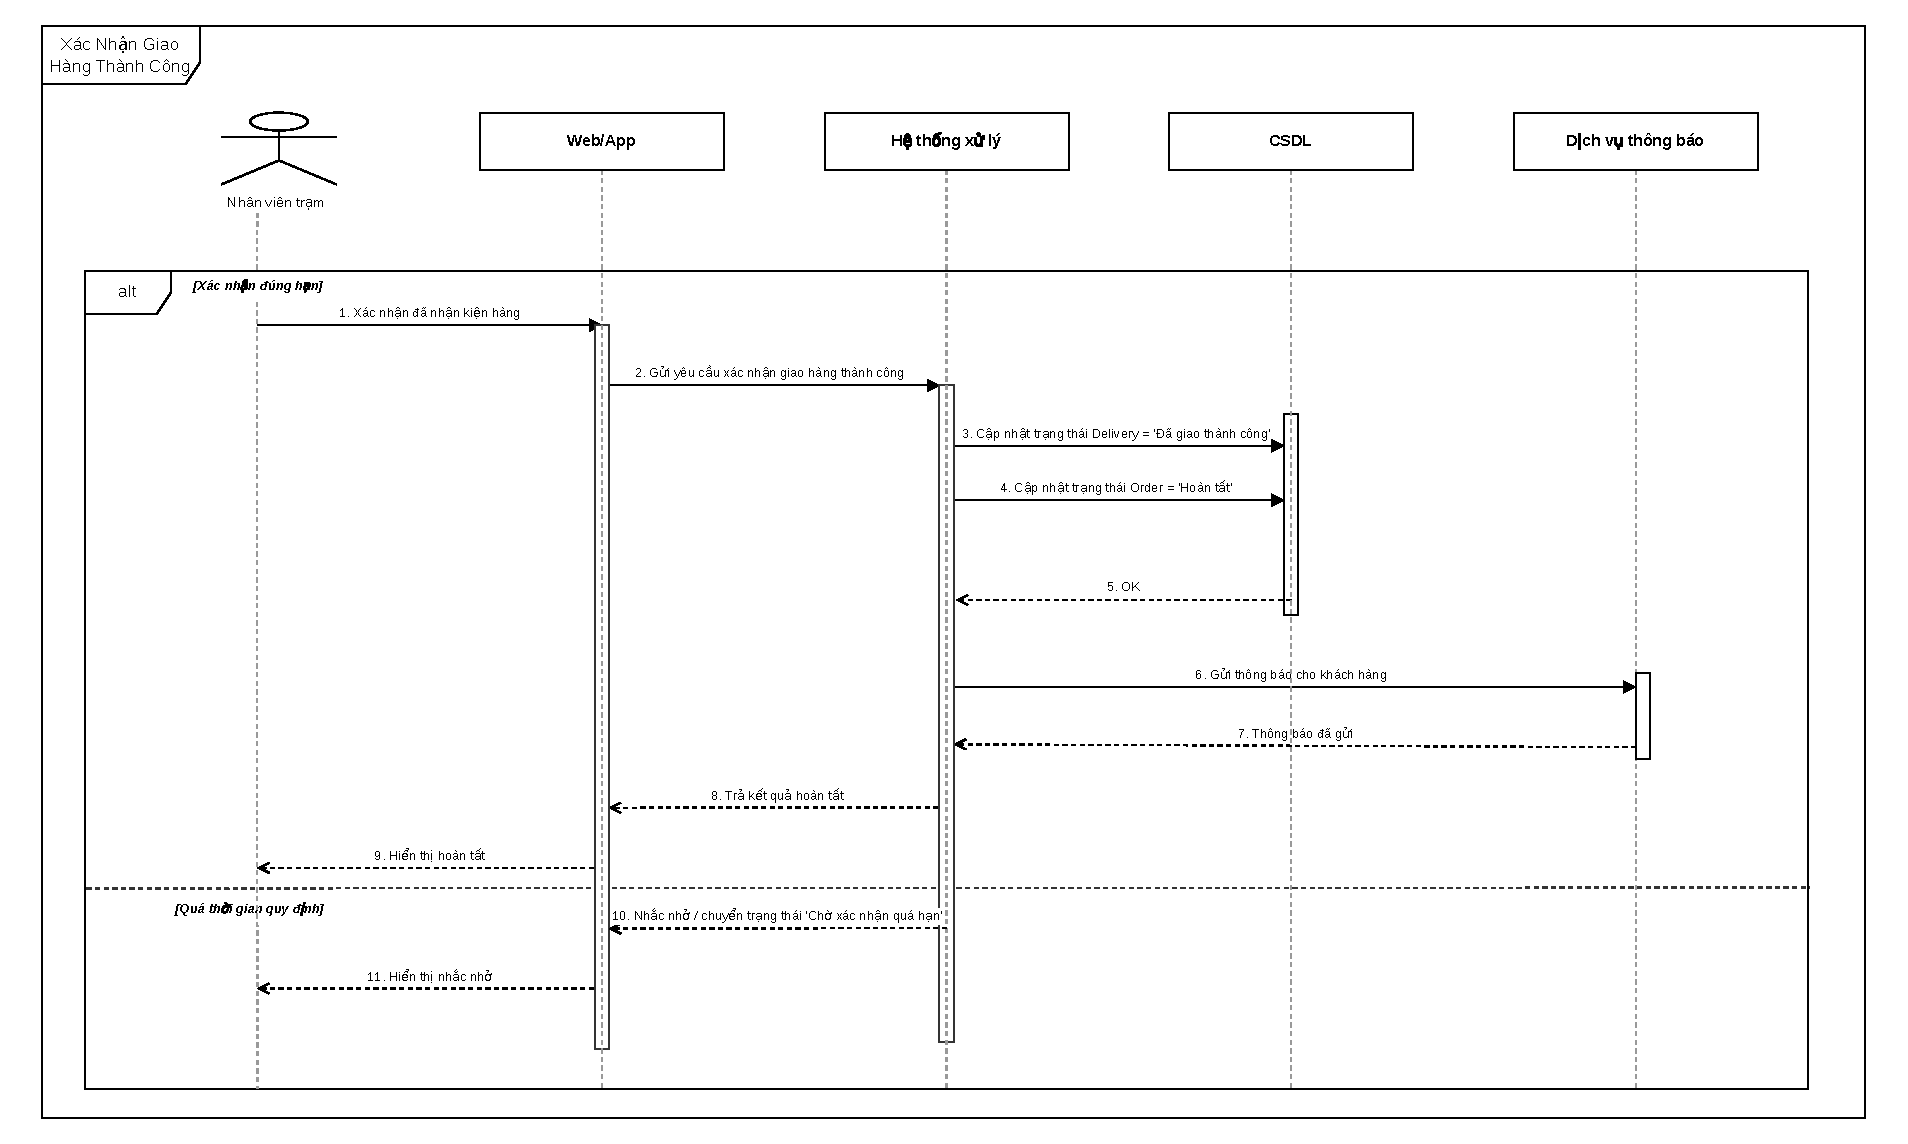
\includegraphics[width=\textwidth]{so-do/sodo-tuantu/Xác Nhận Giao Hàng Thành Công.drawio.pdf}
  \caption{Sơ đồ tuần tự chức năng Xác nhận giao hàng thành công}
  \label{fig:seq-xacnhan-giao-hang-thanh-cong}
\end{figure}
